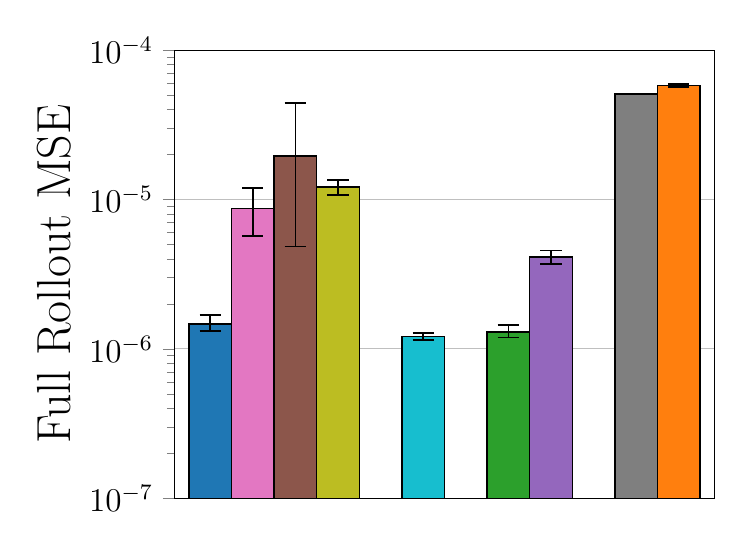
\begin{tikzpicture}
\definecolor{darkgray}{RGB}{169,169,169}
\definecolor{darkorange25512714}{RGB}{255,127,14}
\definecolor{darkslategray38}{RGB}{38,38,38}
\definecolor{darkturquoise23190207}{RGB}{23,190,207}
\definecolor{gray127}{RGB}{127,127,127}
\definecolor{lightgray204}{RGB}{204,204,204}
\definecolor{mediumpurple148103189}{RGB}{148,103,189}
\definecolor{orchid227119194}{RGB}{227,119,194}
\definecolor{sienna1408675}{RGB}{140,86,75}
\definecolor{steelblue31119180}{RGB}{31,119,180}
\definecolor{steelblue76114176}{RGB}{76,114,176}
\definecolor{tabgreen}{RGB}{44,160,44}
\definecolor{olive18818934}{RGB}{188,189,34}

\begin{semilogyaxis}[
  xmin=-0.5, xmax=7.1,
  xtick=\empty,
  ymin=1e-7, ymax=1e-4,
  ymajorgrids,
  tick align=outside,
  ylabel={Full Rollout MSE},
  ylabel style={font=\LARGE},
  ytick pos=left,
  tick label style={font=\large},
]

% Group 1: PEACH (0), pstnet (0.6), gnn_encoder (1.2), test_opt (1.8)
\draw[fill=steelblue31119180, draw=black, line width=0.5pt] (axis cs:-0.3, 1e-7) rectangle (axis cs:0.3,  1.4707e-6);
\draw[fill=orchid227119194,   draw=black, line width=0.5pt] (axis cs:0.3,  1e-7) rectangle (axis cs:0.9,  8.7298e-6);
\draw[fill=sienna1408675,     draw=black, line width=0.5pt] (axis cs:0.9,  1e-7) rectangle (axis cs:1.5,  1.9537e-5);
\draw[fill=olive18818934,     draw=black, line width=0.5pt] (axis cs:1.5,  1e-7) rectangle (axis cs:2.1,  1.2119e-5);

% Group 2: MaNGO (3.0)
\draw[fill=darkturquoise23190207, draw=black, line width=0.5pt] (axis cs:2.7, 1e-7) rectangle (axis cs:3.3, 1.2112e-6);

% Group 3: Oracle (4.2), Oracle MGN (4.8)
\draw[fill=tabgreen,              draw=black, line width=0.5pt] (axis cs:3.9, 1e-7) rectangle (axis cs:4.5, 1.2985e-6);
\draw[fill=mediumpurple148103189, draw=black, line width=0.5pt] (axis cs:4.5, 1e-7) rectangle (axis cs:5.1, 4.1116e-6);

% Group 4: No Context (6.0), No Context MGN (6.6)
\draw[fill=gray127,            draw=black, line width=0.5pt] (axis cs:5.7, 1e-7) rectangle (axis cs:6.3, 5.0834e-5);
\draw[fill=darkorange25512714, draw=black, line width=0.5pt] (axis cs:6.3, 1e-7) rectangle (axis cs:6.9, 5.7853e-5);

% Error bars
% PEACH (center 0)
\draw[black, semithick] (axis cs:0,    1.3136e-6) -- (axis cs:0,    1.6826e-6);
\draw[black, semithick] (axis cs:-0.15,1.3136e-6) -- (axis cs:0.15, 1.3136e-6);
\draw[black, semithick] (axis cs:-0.15,1.6826e-6) -- (axis cs:0.15, 1.6826e-6);
% pstnet (center 0.6)
\draw[black, semithick] (axis cs:0.6,  5.6903e-6) -- (axis cs:0.6,  1.1975e-5);
\draw[black, semithick] (axis cs:0.45, 5.6903e-6) -- (axis cs:0.75, 5.6903e-6);
\draw[black, semithick] (axis cs:0.45, 1.1975e-5) -- (axis cs:0.75, 1.1975e-5);
% gnn_encoder (center 1.2)
\draw[black, semithick] (axis cs:1.2,  4.8388e-6) -- (axis cs:1.2,  4.4339e-5);
\draw[black, semithick] (axis cs:1.05, 4.8388e-6) -- (axis cs:1.35, 4.8388e-6);
\draw[black, semithick] (axis cs:1.05, 4.4339e-5) -- (axis cs:1.35, 4.4339e-5);
% test_opt (center 1.8)
\draw[black, semithick] (axis cs:1.8,  1.0742e-5) -- (axis cs:1.8,  1.3495e-5);
\draw[black, semithick] (axis cs:1.65, 1.0742e-5) -- (axis cs:1.95, 1.0742e-5);
\draw[black, semithick] (axis cs:1.65, 1.3495e-5) -- (axis cs:1.95, 1.3495e-5);
% MaNGO (center 3.0)
\draw[black, semithick] (axis cs:3.0,  1.1531e-6) -- (axis cs:3.0,  1.2742e-6);
\draw[black, semithick] (axis cs:2.85, 1.1531e-6) -- (axis cs:3.15, 1.1531e-6);
\draw[black, semithick] (axis cs:2.85, 1.2742e-6) -- (axis cs:3.15, 1.2742e-6);
% oracle (center 4.2)
\draw[black, semithick] (axis cs:4.2,  1.1952e-6) -- (axis cs:4.2,  1.4497e-6);
\draw[black, semithick] (axis cs:4.05, 1.1952e-6) -- (axis cs:4.35, 1.1952e-6);
\draw[black, semithick] (axis cs:4.05, 1.4497e-6) -- (axis cs:4.35, 1.4497e-6);
% mgn_oracle (center 4.8)
\draw[black, semithick] (axis cs:4.8,  3.7078e-6) -- (axis cs:4.8,  4.5653e-6);
\draw[black, semithick] (axis cs:4.65, 3.7078e-6) -- (axis cs:4.95, 3.7078e-6);
\draw[black, semithick] (axis cs:4.65, 4.5653e-6) -- (axis cs:4.95, 4.5653e-6);
% No Context (center 6.0)
\draw[black, semithick] (axis cs:6.0,  5.0709e-5) -- (axis cs:6.0,  5.0959e-5);
\draw[black, semithick] (axis cs:5.85, 5.0709e-5) -- (axis cs:6.15, 5.0709e-5);
\draw[black, semithick] (axis cs:5.85, 5.0959e-5) -- (axis cs:6.15, 5.0959e-5);
% No Context MGN (center 6.6)
\draw[black, semithick] (axis cs:6.6,  5.6436e-5) -- (axis cs:6.6,  5.9399e-5);
\draw[black, semithick] (axis cs:6.45, 5.6436e-5) -- (axis cs:6.75, 5.6436e-5);
\draw[black, semithick] (axis cs:6.45, 5.9399e-5) -- (axis cs:6.75, 5.9399e-5);

\end{semilogyaxis}
\end{tikzpicture}